%**************************************************************************************
% License:
% CC BY-NC-SA 4.0 (http://creativecommons.org/licenses/by-nc-sa/4.0/)
%**************************************************************************************

\documentclass[notes]{beamer}

\mode<presentation> {

\usetheme{Madrid}

% Burnt orange
\definecolor{burntorange}{rgb}{0.8, 0.33, 0.0}
\colorlet{beamer@blendedblue}{burntorange}
% Pale yellow
\definecolor{paleyellow}{rgb}{1.0, 1.0, 0.953}
\setbeamercolor{background canvas}{bg=paleyellow}
% Secondary and tertiary palett
\setbeamercolor*{palette secondary}{use=structure,fg=white,bg=burntorange!80!black}
\setbeamercolor*{palette tertiary}{use=structure,fg=white,bg=burntorange!60!black}

% To remove the footer line in all slides uncomment this line
%\setbeamertemplate{footline}
% To replace the footer line in all slides with a simple slide count uncomment this line
%\setbeamertemplate{footline}[page number]

% To remove the navigation symbols from the bottom of all slides uncomment this line
%\setbeamertemplate{navigation symbols}{}
}

\usepackage{amsmath}
\usepackage{bm}
\usepackage{breqn}
\usepackage{cancel}
\usepackage{graphicx} % for figures
\usepackage{subcaption} % for subplots 
\usepackage[labelsep=space,tableposition=top]{caption}
\renewcommand{\figurename}{Fig.} 
\usepackage{cleveref}
\usepackage{caption,subcaption}% http://ctan.org/pkg/{caption,subcaption}
\usepackage{booktabs} % Allows the use of \toprule, \midrule and \bottomrule in tables
\usepackage{multirow}
\usepackage{tabularx}
\usepackage{siunitx}
\usepackage{cleveref}
\usepackage{xcolor}
\usepackage{empheq}
\usepackage[most]{tcolorbox}

\newtcbox{\mymath}[1][]{%
	nobeforeafter, math upper, tcbox raise base,
	enhanced, colframe=blue!30!black,
	colback=blue!30, boxrule=1pt,
	#1}

% To print 2 slides on a page
%\usepackage{handoutWithNotes}
%\pgfpagesuselayout{2 on 1}[border shrink=2mm]
%----------------------------------------------------------------------------------------
%	TITLE PAGE
%----------------------------------------------------------------------------------------
% The short title appears at the bottom of every slide, the full title is only on the title page
\title[CE394M: Stress-strain-strength]{CE394M: Stress-strain-strength relationship of clay} 
\author{Krishna Kumar} % name
\institute[UT Austin] % institution 
{
University of Texas at Austin \\
\medskip
\textit{
  \url{krishnak@utexas.edu}} % Your email address
}
\date{\today} % Date, can be changed to a custom date

\begin{document}

\begin{frame}
\titlepage % title page as the first slide
\end{frame}

\begin{frame}
 % Table of contents slide, comment this block out to remove it
 \frametitle{Overview}
  %Throughout your presentation, if you choose to use \section{} and \subsection{} 
  %commands, these %will automatically be printed on this slide as an overview 
 \tableofcontents
\end{frame}

%----------------------------------------------------------------------------------------
% slides
%----------------------------------------------------------------------------------------
\section{Stress-strain-strength relationship}
%----------------------------------------------------------------------------------------
\begin{frame}
\frametitle{L-soil v D-soil}
L-soils:
\mode<beamer>{
	\begin{itemize}
		\item yield at sub-critical stress ratios
		\item looser than their critical density at their projected yield stress
		\item lightly over-consolidated at yield
		\item contractile when sheared slowly
		\item ``wet" when sheared quickly
		\item tend to strain-harden to a critical state if sheared beyond yield point
	\end{itemize}
}
\mode<handout>{
	\vspace{3cm}
}
D-soils:
\mode<beamer>{
	\begin{itemize}
		\item fail at super-critical stress ratios
		\item denser than their critical density at their projected yield stress
		\item heavily over-consolidated at yield
		\item dilatant when sheared slowly
		\item ``dry" when sheared quickly
		\item tend to strain-soften to a critical state if sheared beyond yield point
	\end{itemize}
}
\mode<handout>{
	\vspace{3cm}
}
\end{frame}
\note{The terms ``wet" and ``dry" come from the idea of working a specimen of soil by hand. On the wet side of critical state the soil skeleton is too loosely compacted to support pressure stress—such stress, if applied (such as by squeezing the soil by hand) passes immediately into the pore water and thus causes this water to bleed out of the specimen and wet the hands. The opposite effect occurs when the soil is on the dry side of critical state.}

%----------------------------------------------------------------------------------------
\section{Simple shear}
%----------------------------------------------------------------------------------------
\begin{frame}
\frametitle{Simple shear}
	\begin{figure}
		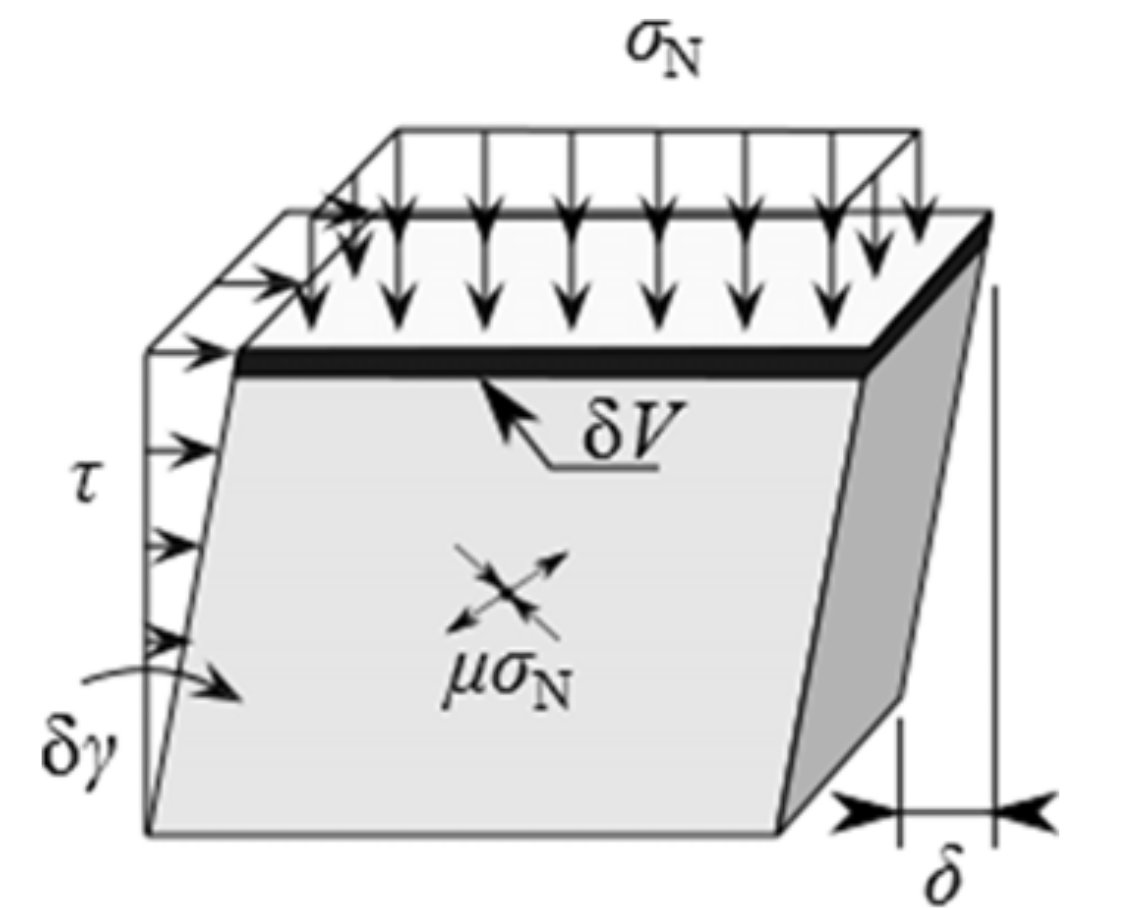
\includegraphics[width=0.9\textwidth]{figs/simple-shear.png}
	\end{figure}
\end{frame}

%----------------------------------------------------------------------------------------
\begin{frame}
\frametitle{Simple shear: Normally Consolidated Clay - L-soil}
\mode<beamer>{
	\begin{figure}
		\includegraphics[width=0.65\textwidth]{figs/ncl.png}
		\caption*{Drained shear: $L \rightarrow L_d$ and $\delta u = 0$. Undrained shear: $L \rightarrow L_u$ and $\delta v = 0$.}
	\end{figure}
}
\mode<handout>{
	\vspace{6cm}
}
\end{frame}

%----------------------------------------------------------------------------------------
\begin{frame}
\frametitle{NCL: L-soil (drained v undrained)}
\mode<beamer>{
	\begin{figure}
		\includegraphics[width=0.9\textwidth]{figs/ncl-1.png}
	\end{figure}
}
\mode<handout>{
	\vspace{6cm}
}
\end{frame}
\note{
	Note that the stack of $\kappa-$lines with their associated Cam Clay yield surfaces creates a 3D boundary surface in $(\tau, \sigma^\prime, v)$ space.
	
	State paths starting inside the boundary surface begin as elastic until they hit the surface.
	Then they are forced to follow the boundary surface, obeying whatever test constraint is
	imposed (undrained v = const, or drained $\sigma^\prime$ = const) until the
	path reaches the critical state
	line. Then the soil shears at
	constant $(\tau, \sigma^\prime, v)$ state.
	
	VCL: $d\varepsilon_p^e + d\varepsilon_p^p$ Elasto-plastic yielding
	RCL: $d\varepsilon_p^e$ only elastic
	
	Isotropic loading along VCL ($q = 0$) can develop plastic strains: essentially hardening cap.
	
	VCL: $N - \lambda \ln p^\prime \quad \eta = 0$
	RCL: $\Gamma - \lambda \ln p^\prime \quad \eta = M$
	$N = \Gamma + (\lambda - \kappa)$

}

%----------------------------------------------------------------------------------------
\begin{frame}
\frametitle{SS: LOC-soil (L-soils)}
\mode<beamer>{
	\begin{figure}
		\includegraphics[width=0.65\textwidth]{figs/loc.png}
	\end{figure}
}
\mode<handout>{
	\vspace{6cm}
}
\end{frame}
\note{
	In undrained conditions, the effective stress path
	will be $d\sigma^\prime = 0$ during elastic response.
	
	$d\sigma^\prime = (vp^\prime / \kappa) d\varepsilon_v$.
	
	$d\varepsilon_v = 0$ hence $d\sigma^\prime = 0$.
}

%----------------------------------------------------------------------------------------
\begin{frame}
\frametitle{SS: LOC-soil (L-soils)  (drained v undrained)}
\mode<beamer>{
	\begin{figure}
		\includegraphics[width=0.9\textwidth]{figs/loc-1.png}
	\end{figure}
}
\mode<handout>{
	\vspace{6cm}
}
\end{frame}

%----------------------------------------------------------------------------------------
\begin{frame}
\frametitle{SS: HOC-soil (D-soils)}
\mode<beamer>{
	\begin{figure}
		\includegraphics[width=0.75\textwidth]{figs/hoc.png}
	\end{figure}
}
\mode<handout>{
	\vspace{6cm}
}
\end{frame}

%----------------------------------------------------------------------------------------
\begin{frame}
\frametitle{SS: HOC-soil (D-soils)  (drained v undrained)}
\mode<beamer>{
\begin{figure}
	\includegraphics[width=0.9\textwidth]{figs/hoc-1.png}
\end{figure}
}
\mode<handout>{
\vspace{6cm}
}
\end{frame}

%----------------------------------------------------------------------------------------
\begin{frame}
\frametitle{TXC: Drained strength and volume at failure using CS}
\begin{figure}
	\includegraphics[width=0.9\textwidth]{figs/txc.png}
\end{figure}
\end{frame}

%----------------------------------------------------------------------------------------
\begin{frame}
\frametitle{TXC: Drained (Mohr-Coulomb ESA)}
\begin{figure}
	\includegraphics[width=0.9\textwidth]{figs/mc-txc-drained.png}
\end{figure}
\end{frame}

%----------------------------------------------------------------------------------------
\begin{frame}
\frametitle{TXC: Drained Cam-Clay yield and failure}
\begin{figure}
	\includegraphics[width=0.9\textwidth]{figs/drained-txc.png}
\end{figure}
\end{frame}

%----------------------------------------------------------------------------------------
\begin{frame}
\frametitle{TXC Drained (axial loading)}
\mode<beamer>{
	\begin{figure}
		\includegraphics[width=0.78\textwidth]{figs/txc-drained.png}
	\end{figure}
}
\mode<handout>{
	\vspace{6cm}
}
\end{frame}
\note{
	The total stress path of triaxial compression has a slope of 1:3. In drained test, the pore
	pressure is kept constant. Hence, the
	effective stress path will have a slope of 1:3.
}

%----------------------------------------------------------------------------------------
\begin{frame}
\frametitle{TXC Drained (axial loading)}
\mode<beamer>{
	\begin{figure}
		\includegraphics[width=0.8\textwidth]{figs/txc-drained-1.png}
	\end{figure}
}
\mode<handout>{
	\vspace{6cm}
}
\end{frame}

%----------------------------------------------------------------------------------------
\begin{frame}
\frametitle{TXC: Undrained strength and excess PWP at failure}
\begin{figure}
	\includegraphics[width=0.9\textwidth]{figs/undrained-txc.png}
\end{figure}
\end{frame}

%----------------------------------------------------------------------------------------
\begin{frame}
\frametitle{TXC: Undrained (Mohr-Coulomb ESA)}
\begin{figure}
	\includegraphics[width=0.9\textwidth]{figs/mc-txc-undrained.png}
\end{figure}
\end{frame}

%----------------------------------------------------------------------------------------
\begin{frame}
\frametitle{TXC Undrained (axial loading)}
\mode<beamer>{
	\begin{figure}
		\includegraphics[width=0.8\textwidth]{figs/txc-undrained.png}
	\end{figure}
}
\mode<handout>{
	\vspace{6cm}
}
\end{frame}

\note{
	Elastic deformation: $dp^\prime = K d\varepsilon_v$ and $dq = 3 G d\varepsilon_s$.
	
	\begin{align*}
	K & = \frac{v p^\prime}{\kappa} \\
	G & = \frac{3K (1 - 2 \nu)}{2(1+\nu)}
	\end{align*}
	
	In undrained conditions, the effective stress path
	will be $dp^\prime = 0$ during elastic response.
	
	\begin{equation*}
	d\varepsilon_v = 0 \quad dp^\prime = 0
	\end{equation*}
}

%----------------------------------------------------------------------------------------
\begin{frame}
\frametitle{TXC Undrained (axial loading)}
\mode<beamer>{
	\begin{figure}
		\includegraphics[width=0.8\textwidth]{figs/txc-undrained-1.png}
	\end{figure}
}
\mode<handout>{
	\vspace{6cm}
}
\end{frame}

%----------------------------------------------------------------------------------------
\begin{frame}
\frametitle{Critical state concept}
\begin{figure}
	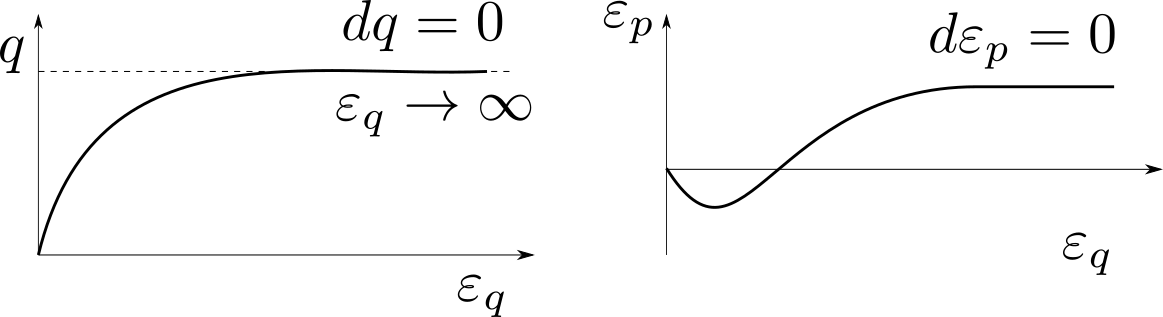
\includegraphics[width=\textwidth]{figs/critical-state.png}
\end{figure}
\end{frame}
\note{The critical state concept shows that undrained shear strength is purely a function of initial void ratio (or water content).}


%----------------------------------------------------------------------------------------
\begin{frame}
\frametitle{Critical state concept}
Interchangeable parameters for stress at yield and $d\varepsilon^p$.
\begin{figure}
	\includegraphics[width=\textwidth]{figs/cam-clay.png}
\end{figure}
Plastic work and dissipation: $\sigma^* \partial \varepsilon^* + \tau^* \partial \gamma^* = \mu_{crit}^* \sigma^* \partial \gamma^*$.

General yield surface: $\frac{\tau^*}{\sigma^*} = \mu^* = \mu^*_{crit} \ln \left[\frac{\sigma_c^*}{\sigma}\right]$
\end{frame}


%----------------------------------------------------------------------------------------
\begin{frame}
\frametitle{Critical state concept: 1D compression}
\begin{figure}
	\includegraphics[width=0.7\textwidth]{figs/1d-compression.png}
\end{figure}
Plastic compression stress $\sigma_c^\prime$ is taken as the larger of the initial aggregate crushing stress and the historic maximum effective vertical stress. Clay muds are taken to begin with $\sigma_c^\prime = 1$kPa.

Plastic compression (normal compression line): $v = v_\lambda - \lambda \ln \sigma^\prime$ for $\sigma^\prime = \sigma^\prime_c$.

Elastic swelling and recompression line ($\kappa-$line): $ v = v_c + \kappa (\ln \sigma_c^\prime - \ln \sigma_v^\prime)$. 
\end{frame}
\note{
Equivalent parameters for log 10 stress scale:

Terzaghi’s compression index: $C_c = \lambda \log10 = \lambda \times 2.3026$


Terzaghi’s swelling index: $C_s / C_r = \kappa \log 10 = \lambda \times  2.3026$
}
\end{document}
